%There have been a few approaches to describe the current \cite{Zagoskin1997}, \cite{Barzykin1999} and many many more. What they have in common: integration over the geometry of the current, which follows along straight lines. Idea of summing over channels of momenta, in a way that
\begin{equation}
\sum_\mathbf{\kappa} \frac{2 e v_{Fx}}{\pi L}
\end{equation}
Expression for current, integrated along the trajectory from a recent publication \cite{Meier2016}:
\begin{equation}
\int_{-W/2}^{+W/2} dy \int_{-p_F}^{+p_F} \frac{dp_y}{2 \pi} \frac{L}{\tilde{L}} \mathcal{J} \left( \chi, \phi \right)
\end{equation}
A trajectory connecting the superconducting interfaces, illustrated in see figure (\ref{fig:sns-parametrisation}), can be parametrized by 
\begin{equation}
\tan \theta = \frac{y_2 - y_1}{L}
\label{eq:parametrization}
\end{equation}
with $\theta$ being the angle between the trajectory and the x-axis.
The x-component of a trajectory is expressed with this angle $\theta$. 
\begin{equation}
v_F = v_{F,x} \cos \theta
\end{equation}

\begin{equation}
\mathcal{J}^s (\chi) = \frac{\mathcal{T} \sin \chi}{\sqrt{1 - \mathcal{T} \sin^2 \frac{\chi}{2}}}
\end{equation}

\begin{equation}
\mathcal{J}^l(\chi) = \sum_{k = 1}^{\infty} \frac{(-1)^{k+1}}{k} \sin( k \chi).
\end{equation}
%%%%%%
Current density for short and long junction limit: 
In the short junction limit the current density can be derived from the scattering matrix formalism and it reads
\begin{equation}
\mathcal{J}^s (\chi) = \frac{\mathcal{T} \sin \chi}{\sqrt{1 - \mathcal{T} \sin^2 \frac{\chi}{2}}}
\end{equation}
$\mathcal{T}$ is the transmission coefficient that describes the transmission through a channel (each channel corresponds to a eigenvalue of the scattering matrix.
The current density for the long junction limit is
\begin{equation}
\mathcal{J}(\chi) = \sum_{k = 1}^{\infty} \frac{(-1)^{k+1}}{k} \sin( k \chi).
\end{equation}
\begin{figure}
\centering
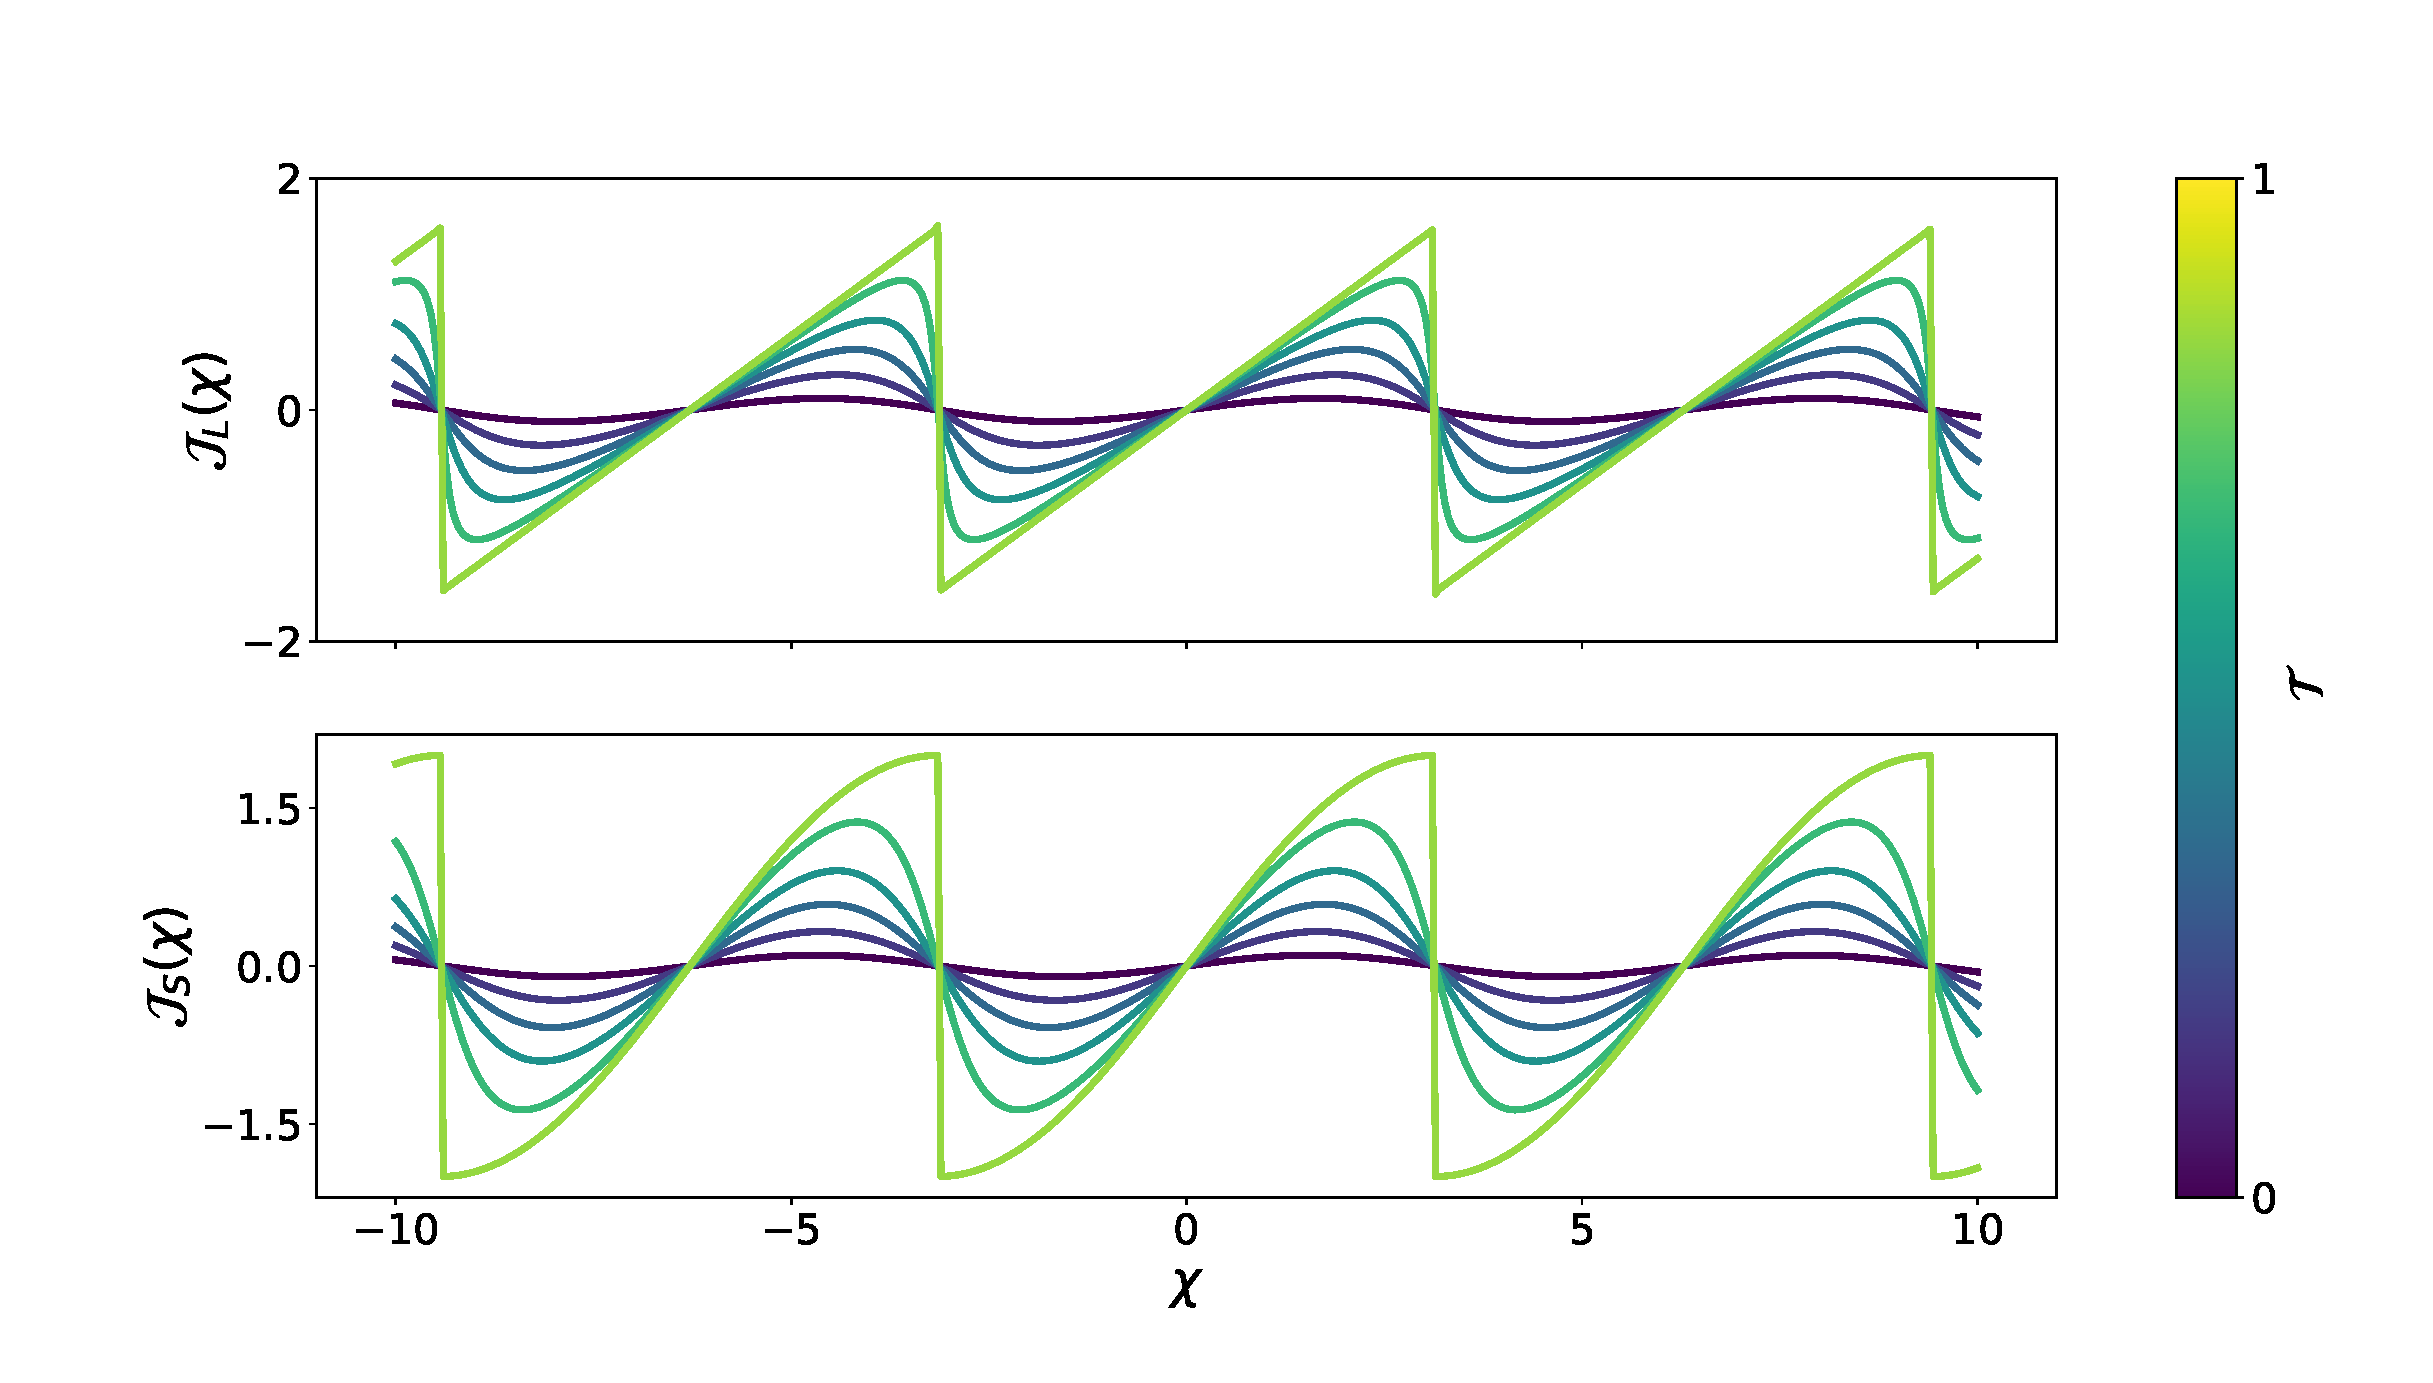
\includegraphics[width=\textwidth]{figure/analyticalmodel/current_density_all}
\caption{Short and long junction current density}
\label{fig:current_density}
\end{figure}
Figure \ref{fig:current_density} shows a plot of both short and long junction limit current densities. They differ for a large transmission coefficient $\mathcal{T} \simeq 1$, where in the long junction limit we observe a sawtooth like shape and in the short junction limit we have a sinusoidal shape.\\
Using the current density the Josephson current at zero magnetic field ($\phi = 0$) can be expressed as 
\begin{equation}
J\left(\chi, \phi=0\right) = \frac{2 e v_F}{\pi \lambda_F L^2}  \int \int_{-W/2}^{W/2} d y_1 d y_2 \frac{\mathcal{J}(\chi)}{\left[ 1 + \left(\frac{y_1 - y_2}{L}\right)^2\right]^2}
\label{eq:josephson_current_zero_b}
\end{equation}
\subsection*{Including magnetic field}
\textbf{Include parametrizaation of trajectories somewhere, important for calculation of magnetic phase!}\\
So far, the current has been derived for zero magnetic field. If a finite magnetic field is considered, the phase $\chi$ will be modified because of two effects. The magnetic phase that will be acquired along a trajectory connecting two points $y_1$ and $y_2$  leads to an additional term in the phase. Then again, \textit{the condition of zero screening current in the bulk superconducting region and the limit of} $\lambda_L \rightarrow 0$ \textit{require the superconducting phase at the interfaces to become functions of y.}\\
\textbf{TODO: Umschreiben!}\\
\begin{eqnarray}
\chi_{1/2} &=& \mp \frac{1}{2}\left( \chi - \frac{2 \pi B L }{\phi_0} y_{1/2}\right) \\
\tilde{\chi}(y_1, y_2) &=& \chi_2 - \chi_1 \\
 &=& \chi - \frac{\pi B L}{\phi_0}(y_1 + y_2)
 \label{eq:chi}
\end{eqnarray}
Assuming that the London penetration depth is small to zero in the superconducting regions the following gauge for the vector potential can be used
\begin{equation}
\mathbf{A}=A_y \mathbf{e}_y, \quad
A_y=\left\{ 
		\begin{array}{ll}
				-B x, & -L/2 \leq x \leq L/2, \\[0.2cm] 
				-\frac{1}{2} B L |x| , & \quad |x|>L/2
		\end{array} 
	\right.
\label{eq:Ay}
\end{equation}
This gauge will give no additional contribution to the phase on straight trajectories
\begin{eqnarray}
\delta \chi &=& \frac{2 \pi}{\Phi_0} \int d \mathbf{l} \cdot \mathbf{A} \\
&=& \frac{2 \pi}{\Phi_0} \int_{-L/2}^{L/2} \frac{dx}{\cos \theta} A_y (x) \sin \theta \\
&=& - \frac{2 \pi B}{\Phi_0} \frac{y_2 - y_1}{L} \int_{-L/2}^{L/2} x dx \\
&=& 0, 
\end{eqnarray}
where eq~(\ref{eq:parametrization}) has been used. The total phase for this setup therefore is eq.~(\ref{eq:chi}). This mean that the current phase relation in the expression for the Josephson current from eq. (\ref{eq:josephson_current_zero_b}) for zero magnetic field has to replaced by the effective phase $\chi \rightarrow \tilde{\chi}(y_1, y_2)$ and then reads
\begin{equation}
J\left(\chi, \phi \right) = \frac{2 e v_F}{\pi \lambda_F L^2}  \int \int_{-W/2}^{W/2} d y_1 d y_2 \frac{\mathcal{J}(\tilde{\chi}(y_1, y_2))}{\left[ 1 + \left(\frac{y_1 - y_2}{L}\right)^2\right]^2}
\label{eq:josephson_current}
\end{equation}
By maximizing the Josephson current with respect to $\chi$, the critical current can be found:
\begin{equation}
I_c(\phi) = \text{max}_{\chi}\left\{ J(\chi, \phi) \right\}
\end{equation}
\textbf{TODO: Dependence on W/L ratio? Plot of current?}
